%% For double-blind review submission, w/o CCS and ACM Reference (max submission space)
\documentclass[10pt,conference]{ieeetran}%\settopmatter{printfolios=true,printccs=false,printacmref=false}

\usepackage{booktabs}   %% For formal tables:
                        %% http://ctan.org/pkg/booktabs
\usepackage{subcaption} %% For complex figures with subfigures/subcaptions
                        %% http://ctan.org/pkg/subcaption
\usepackage{amsmath,amsthm,amssymb}

\usepackage{xcolor,listings}

\usepackage{multirow}

\usepackage{stmaryrd}

\usepackage[noadjust]{cite}

\theoremstyle{definition}
\newtheorem{definition}{Definition}

\newif\ifdraft \drafttrue
\newif\iftext \textfalse
\newif\iflater \latertrue
\newif\ifaftersubmission \aftersubmissionfalse

% !!! PLEASE DON'T CHANGE THESE !!! INSTEAD DEFINE YOUR OWN texdirectives.tex !!!
\makeatletter \@input{texdirectives} \makeatother

%\IEEEoverridecommandlockouts
% The preceding line is only needed to identify funding in the first footnote. If that is unneeded, please comment it out.
\usepackage{cite}
\usepackage{amsmath,amssymb,amsfonts}
\usepackage{algorithmic}
\usepackage{hyperref}
\usepackage{graphicx}
\usepackage{textcomp}
\usepackage[capitalize]{cleveref}
\usepackage[inline]{enumitem}

\usepackage{xcolor}
\newcommand{\bcp}[1]{\ifdraft\textcolor{violet}{{[BCP:~#1]}}\fi}
\newcommand{\leo}[1]{\ifdraft\textcolor{teal}{{[LEO:~#1]}}\fi}
\newcommand{\apt}[1]{\ifdraft\textcolor{blue}{{[APT:~#1]}}\fi}
\newcommand{\rb}[1]{\ifdraft\textcolor{orange}{{[RB:~#1]}}\fi}
\newcommand{\sna}[1]{\ifdraft\textcolor{green}{{[SNA:~#1]}}\fi}
\newcommand{\COQ}[1]{\ifdraft\textcolor{red}{{[COQ DIFFERENCE:~#1]}}\fi}

\usepackage{listings}


\usepackage{xspace}
\newcommand{\cn}{\ifdraft\textsuperscript{\textcolor{blue}{[citation needed]}}\xspace\fi}

\makeatletter
\begingroup
\lccode`\A=`\-
\lccode`\N=`\N
\lccode`\V=`\V
\lowercase{\endgroup\def\memory@noval{ANoValue-}}
\long\def\memory@fiBgb\fi#1#2{\fi}
\long\def\memory@fiTBb\fi#1#2#3{\fi#2}
\newcommand\memory@ifnovalF[1]%>>=
  {%
    \ifx\memory@noval#1%
      \memory@fiBgb
    \fi
    \@firstofone
  }%=<<
\newcommand\memory@ifnovalTF[1]%>>=
  {%
    \ifx\memory@noval#1%
      \memory@fiTBb
    \fi
    \@secondoftwo
  }%=<<
\newcommand\memory@Oarg[2]%>>=
  {%
    \@ifnextchar[{\memory@Oarg@{#2}}{#2{#1}}%
  }%=<<
\long\def\memory@Oarg@#1[#2]%>>=
  {%
    #1{#2}%
  }%=<<
\newcommand*\memory@oarg%>>=
  {%
    \memory@Oarg\memory@noval
  }%=<<
\newcommand*\memory@ifcoloropt%>>=
  {%
    \@ifnextchar[\memory@ifcoloropt@true\memory@ifcoloropt@false
  }%=<<
\long\def\memory@ifcoloropt@true#1\memory@noval#2#3%>>=
  {%
    #2%
  }%=<<
\long\def\memory@ifcoloropt@false#1\memory@noval#2#3%>>=
  {%
    #3%
  }%=<<
\newlength\memory@width
\newlength\memory@height
\setlength\memory@width{23pt}
\setlength\memory@height{14pt}
\newcount\memory@num
\newcommand*\memory@blocks[2]%>>=
  {%
    \memory@num#1\relax
    \fboxsep-\fboxrule
    \memory@ifcoloropt#2\memory@noval
      {\def\memory@color{\textcolor#2}}
      {\def\memory@color{\textcolor{#2}}}%
    \loop
    \ifnum\memory@num>0
      \fbox{\memory@color{\rule{\memory@width}{\memory@height}}}%
      \kern-\fboxrule
      \advance\memory@num\m@ne
    \repeat
  }%=<<
% memory:
%  [#1]: width
%   #2 : count
%  [#3]: height
%   #4 : colour
%  [#5]: label
\newcommand*\memory%>>=
  {%
    \begingroup
    \memory@oarg\memory@a
  }%=<<
\newcommand*\memory@a[2]%>>=
  {%
    % #1 width
    % #2 count
    \memory@ifnovalF{#1}{\memory@width#1\relax}%
    \memory@Oarg\memory@height{\memory@b{#2}}%
  }%=<<
\newcommand*\memory@b[3]%>>=
  {%
    % #1 count
    % #2 height
    % #3 colour
    \memory@ifnovalF{#2}{\memory@height#2\relax}%
    \memory@oarg{\memory@c{#1}{#3}}%
  }%=<<
\newcommand*\memory@c[3]%>>=
  {%
    % #1 count
    % #2 colour
    % #3 label
    \memory@ifnovalTF{#3}
      {\ensuremath{\memory@blocks{#1}{#2}}}
      {\ensuremath{\underbrace{\memory@blocks{#1}{#2}}_{\text{#3}}}}%
    \endgroup
  }%=<<
\makeatother

\newcommand{\judgment}[2]{
  {\centering
  \vspace{\abovedisplayskip}
  \begin{tabular}{c}
    #1 \\
    \hline
    #2
  \end{tabular}
   \vspace{\abovedisplayskip}\par}}

\newcommand{\judgmentbr}[4]{
  {\centering
  \vspace{\abovedisplayskip}
  \begin{tabular}{c}
    #1 \\
    #2 \\
    #3 \\
    \hline
    #4
  \end{tabular}
   \vspace{\abovedisplayskip}\par}}


\newcommand{\judgmenttwo}[3]{
  {\centering
  \vspace{\abovedisplayskip}
  \begin{tabular}{c c}
    #1 & #2 \\
    \hline
    \multicolumn{2}{c}{#3}
  \end{tabular}
  \vspace{\abovedisplayskip}\par}}

\newcommand{\judgmentthree}[4]{
  {\centering
  \vspace{\abovedisplayskip}
  \begin{tabular}{c c c}
    #1 & #2 & #3 \\
    \hline
    \multicolumn{3}{c}{#4}
  \end{tabular}
  \vspace{\abovedisplayskip}\par}}

% Notational conventions
\newcommand{\HIGHSEC}{\textsc{HC}}
\newcommand{\LOWSEC}{\textsc{LC}}
\newcommand{\HIGHINT}{\textsc{HI}}
\newcommand{\LOWINT}{\textsc{LI}}
\newcommand{\IDS}{{\mathcal{I}}}
\newcommand{\ID}{I}
\newcommand{\ME}{\textsc{S}}
\newcommand{\NOTME}{\textsc{O}}
\newcommand{\TRANS}{\ensuremath{-}}
\newcommand{\JAL}{\ensuremath{\mathit{JAL}}}
\newcommand{\ACCYES}{\ensuremath{A}}
\newcommand{\ACCNO}{\ensuremath{I}}
\newcommand{\ACCCODE}{\ensuremath{K}}
\newcommand{\CRCALL}{\ensuremath{\mathit{CALL}}}
\newcommand{\CRRET}{\ensuremath{\mathit{RETURN}}}
\newcommand{\CRBOT}{\ensuremath{\bot}}
\newcommand{\VIS}{\textsc{vis}}
\newcommand{\HID}{\textsc{hid}}
\newcommand{\word}{w}
\newcommand{\addr}{a}
\newcommand{\WORDS}{{\mathcal W}}
\newcommand{\reg}{r}
\newcommand{\REGS}{{\mathcal R}}
\newcommand{\mach}{m}
\newcommand{\machT}{M}
\newcommand{\MACHS}{{\mathcal M}}
\newcommand{\MPT}{\mathit{MP}}
\newcommand{\obs}{o}
\newcommand{\obsT}{O}
\newcommand{\OBSS}{\mathit{Obs}}
\newcommand{\PC}[1]{\PCname(#1)}
\newcommand{\PCname}{\textsc{pc}}
\newcommand{\SP}{\textsc{sp}}
\newcommand{\pol}{p}
\newcommand{\POLS}{\mathcal{P}}
\newcommand{\pinit}{pinit}
\newcommand{\prop}{S}
\newcommand{\contour}{C}
\newcommand{\CONTOURS}{{\mathcal C}}
\newcommand{\component}{k}
\newcommand{\COMPONENTS}{{\mathcal K}}
\newcommand{\trace}{T}
\newcommand{\observer}{O}
\newcommand{\stateobs}{\sigma}
\newcommand{\seq}[1]{\overline{#1}}
\newcommand{\SEQ}[1]{\overline{#1}}
\newcommand{\dstk}[1]{{#1}.\mbox{\it stack}}
\newcommand{\dpcd}[1]{{#1}.\mbox{\it PCdepth}}
\newcommand{\ddep}[2]{{#1}.\mbox{\it depth}({#2})}
\newcommand{\dinit}{\mbox{\it Dinit}}
\newcommand{\empstack}{\mbox{\it empty}}
\newcommand{\access}[2]{\mbox{\it accessible}_{#1}({#2})}
\newcommand{\norm}[1]{\lvert{#1}\rvert}
\newcommand{\MPS}{\mathit{MPState}}
\newcommand{\mpstate}[2]{(#1,#2)}
\newcommand{\mpostate}[3]{(#1,#2,#3)}
\newcommand{\mpstatename}{mp}
\newcommand{\callmap}{cm}
\newcommand{\CALLMAPS}{\mathit{CallMap}}
\newcommand{\ret}[1]{\mathit{justret}\ #1}
\newcommand{\nextPC}{next}
\newcommand{\base}{b}
\newcommand{\stepsto}{\Longrightarrow}
\newcommand{\stepstounder}[1]{\stackrel{\mbox{\tiny{$#1$}}}{\Longrightarrow}}
\newcommand{\stepstounderfull}{\stepstounder{\textsc{RISCV}}}
\newcommand{\manystepsto}{\stepsto^\star}
\newcommand{\obstrace}{\mathit{obstrace}}
\newcommand{\funid}{f}
\newcommand{\FUNIDS}{\mathcal{F}}
\newcommand{\retmap}{\mathit{rm}}
\newcommand{\RETMAPS}{\mathit{RetMap}}
\newcommand{\codemap}{\mathit{fm}}
\newcommand{\CODEMAPS}{\mathit{FuncMap}}
\newcommand{\entmap}{\mathit{em}}
\newcommand{\ENTMAPS}{\mathit{EntryMap}}
\newcommand{\PUT}{\mathit{Until}}
\newcommand{\Trace}{T}
\newcommand{\traceelem}{a}
\newcommand{\TRACEELEMS}{A}
\newcommand{\head}{\mathit{head}}
\newcommand{\last}{\mathit{last}}

\newcommand{\stepstoobs}[1]{\xrightarrow{#1}}
\newcommand{\polstep}{\rightharpoonup}
\newcommand{\stepstopol}[1]{\overset{#1}{\rightharpoonup}}
%\newcommand{\stepstopol}[1]{\overset{#1}{\rightharpoonup}_P}

\newcommand{\stepplus}{\Rightarrow}
\newcommand{\stepkappa}{\Rightarrow_\kappa}
\newcommand{\induced}[2]{(#1, #2)^*}
\newcommand{\flows}{\sqsubseteq}
\newcommand{\flowsstrict}{\sqsubset}
\newcommand{\initmach}{\MACHS_{\mathit{init}}}
\newcommand{\initcontour}{\CONTOURS_{\mathit{init}}}
\newcommand{\closure}[1]{\textit{Close}#1}
\newcommand{\variant}[2]{\textit{Vars}(#1, #2)}
\newcommand{\isinf}{\mathit{inf}}

\newcommand{\Last}[1]{\mathit{Last}(#1)}

\newcommand{\HALT}{\textsc{HALT}}

\newcommand{\underscore}{\mbox{\_}}

\newcommand{\propdef}[1]{\text{\sc #1}}

\newcommand{\TRACE}[1]{\mathit{Trace}~(#1)}
\newcommand{\MTRACE}{\TRACE{\MACHS}}
\newcommand{\MOTRACE}{\TRACE{\MACHS \times \OBSS}}
\newcommand{\MPOTRACE}{\TRACE{\MACHS \times \POLS \times \OBSS}}


\makeatletter
\newcommand{\linebreakand}{%
  \end{@IEEEauthorhalign}
  \hfill\mbox{}\par
  \mbox{}\hfill\begin{@IEEEauthorhalign}
}
\makeatother

\begin{document}

%% Title information
\title{Formalizing Stack Safety as a Security Property}

\author{
  \IEEEauthorblockN{
    Sean Noble Anderson
  }
  \IEEEauthorblockA{
    Portland State University\\
    ander28@pdx.edu\\
  }
  \and
  \IEEEauthorblockN{
    Leonidas Lampropoulos
  }
  \IEEEauthorblockA{
    University of Maryland, College Park\\
    leonidas@umd.edu\\
  }
  \and
  \IEEEauthorblockN{
    Roberto Blanco
  }
  \IEEEauthorblockA{
    Max Planck Institute for Security and Privacy\\
    roberto.blanco@mpi-sp.org\\
  }
  \linebreakand
  \IEEEauthorblockN{
    Benjamin C. Pierce
  }
  \IEEEauthorblockA{
    University of Pennsylvania\\
    bcpierce@cis.upenn.edu\\
  }
  \and
  \IEEEauthorblockN{
    Andrew Tolmach
  }
  \IEEEauthorblockA{
    Portland State University\\
    tolmach@pdx.edu\\
  }
}



%% Keywords
%% comma separated list
\ifcameraready
\keywords{Stack Safety, Micro-Policies}  %% \keywords are mandatory in final camera-ready submission
\fi

\maketitle

\section{The Setting}

We state our properties in terms of a generic machine subject to a few constraints,
but our examples and tests are focused on a RISC-V-like machine enhanced with PIPE,
a tag-based reference monitor. Importantly, such a machine has no explicit ``call''
instruction, only {\tt jal} instructions which may be used for that purpose or potentially
other purposes. Similarly, there is no ``return'', only {\tt jalr}, and so on.
We therefore define our properties under the assumption that we can distinguish the
steps that represent these abstract operations from those that do not---for instance,
by labeling instructions as calls, returns, etc.\apt{note proper way to do punctuating dashes}
Such a labeling scheme appears in
our testing environment (Section [TBD]) and is already necessary
to correctly apply tag-based enforcement in practice (cite something about this.)

The set of special operations that are recognized in this way are termed
{\it security operations}. Our properties are phrased as a {\it security semantics},
which extends the underlying machine with additional context about its
security principals and which registers and memory they require to be secure.
This context evolves dynamically through the execution of security operations.
This notion of security may be phrased as
predicates on future states, e.g. assertions of the form
``When control returns to me...'', or relations on traces of future execution
(hyper-properties).

Unlike approaches that give a safe-by-construction semantics
for various security operations and then prove secure compilation to the underlying
enforcement mechanism, our machine is explicitly not safe unless the enforcement
is correctly instantiated; the security semantics gives us the means to judge whether
an enforcement scheme implements stack safety or not. 

We will first give a detailed example of a security semantics for a simple setting
in which our security operations are restricted to making calls and returns, and allocating
private memory within the current function activation. We then extend this model
to the full system that we test, which features:
\begin{itemize}
\item Function calls and returns, with caller- and callee-saved registers
\item Allocation of strictly private and strictly public regions on the stack
\item Arguments spilled onto the stack and/or passed by reference
\item Exceptions
\item Tail-call Elimination
\end{itemize}

Finally, we give a property definition for stack safety in which (some) stack-allocated
objects are governed by a provenance-based capability system, accessible only to those
functions which have recieved a valid pointer to them.

In section (TBD) we discuss the extension of this model into a simple concurrency setup.

\paragraph*{Threat Model}

We must trust that our method of distinguishing security operations is accurate; if it
involves labels placed on code by a compiler, that means trusting that the compiler placed
those labels correctly. If operations occur that are not recognized, those operations
might not be guaranteed to protect their principals---for instance, an unlabeled call
might not protect the caller's data from the callee. On the flip side, applying an incorrect
label most likely means that the property becomes too strong to be enforced.

Otherwise, we do not assume that the code is reasonable\apt{still vague} or adheres to any particular
calling convention or source construct. In particular, while we are agnostic as to the source
language, we certainly aim to support C, and so any source function might contain undefined
behavior resulting in its compilation to arbitrary machine code. A given enforcement
mechanism may place additional constraints, of course, particularly on the behavior of
call and return sequences.

In general, it is impossible to distinguish buggy source code from an attacker; in
our examples we will identify one function or another as an attacker, but we do not
require any static division between trusted and untrusted code, and aim to protect
even buggy code.

This is a strong threat model, but hardware and timing attacks are out of scope,
and our properties are termination insensitive as a result of the enforcement mechanism
(below).

\paragraph*{Limitations}

Our concurrency model is fairly
simplistic, assuming a fixed number of threads each with its own dedicated processor.
We model memory safe stack objects, but not a heap. Regions outside of
stacks can be used however the compiler likes, including as a heap, but no protection is
built in and our properties assume that if a pointer to a stack object is stored there,
it is permanently compromised.

\subsection{The Basic Machine}

The building blocks of the machine are {\em words} and {\em registers}.
Words are ranged over by \(\word\) and, when used as addresses, \(\addr\),
and are drawn from the set \(\WORDS\).
Registers in the set \(\REGS\) are ranged over by \(\reg\), with special names given to the
program counter \(\PCname\) and stack pointer \(\SP\).
They are divided into sets of caller-saved and callee-saved registers;
Figure \ref{fig:RISCVregs} gives an example division for a RISC-V machine as will
appear in our examples and testing, along with the register names that will appear in
example code, and their default security class (explained below).

\begin{figure}
  \begin{tabular}{| l | l | l |}
    \hline
    Set / & Names & Purpose \\
    Class & & \\
    \hline
    \(\mathit{CLR}\) / & {\tt t0} -- {\tt t6} & Caller-saved temps \\
    \(\unsealed\) & {\tt a0} -- {\tt a1} & Caller-saved args / return vals \\
    & {\tt a2} -- {\tt a7} & Caller-saved args \\
    \hline
    \(\mathit{CLE}\) / & {\tt s0} -- {\tt s7} & Callee-saved \\
    \(\sealed\) & {\tt ra} & Return Address \\
    & {\tt sp} & Stack Pointer \\  
    \hline
    \(\mathit{PUBLIC}\) / & {\tt pc} & Program Counter \\
    \(\public\) & & \\
    \hline
  \end{tabular}
  \caption{RISC-V register set}
  \label{fig:RISCVregs}
\end{figure}

Collectively addresses and registers are {\em state elements} \(\component\)
in the set \(\COMPONENTS ::= \WORDS + \REGS\).
%
{\em Machine states} are drawn from a set \(\MACHS\) ranged over by \(\mach\)
that defines a mapping \(\mach[\component]\) from state elements to words.
{\em Events} are drawn from a set \(\OBSS\) and ranged over by \(\obs\), with a
special silent event \(\tau\).
The machine step function
\(\mach \xrightarrow{\overline{\psi},\obs} \mach' \in \MACHS \rightarrow
\MACHS \times \mathit{list} ~ \Psi \times \OBSS\)
is labeled by an ordered list of security operations, defined below,
and an event.
While the tag-based enforcement mechanism may cause the machine to
failstop, we model this as the machine silently diverging by remaining in the
same state. Since failstops are not distinguished from normal execution,
our properties will suffer the limitations typical of
{\it termination insensitive} systems \cite{}. TODO: more detailed explanation later.

For convenience, we will abbreviate multiple updates of a mapping
\(\mach[\component_0 \mapsto \word_0][\component_1 \mapsto \word_1]\dots\)
as \(\mach \llbracket A \mapsto B | C \rrbracket\), where \(A\) and \(B\)
are fomulae with free variables bound to sets in \(C\).

\subsection{Security Operations, Principals, and Security State}

Security operations consist of calls (including tailcalls), returns,
allocations and deallocations. Calls and tailcalls identify the address of the call's target,
and the argument registers. Allocations and deallocations are phrased in terms of a pair
of an offset from the stack pointer and a size. Returns don't require any additional information.
%
\begin{align*}
  \psi \in \Psi ::= & \mathbf{call} ~ \addr_{target} ~ \overline{\reg_{args}} ~ \overline{sa} &
  sa \in \REGS \times \mathbb{Z} \times \mathbb{N} \\
  | & \mathbf{tailcall} ~ \addr_{target}  ~ \overline{\reg_{args}} ~ \overline{sa} &
  sa \in \REGS \times \mathbb{Z} \times \mathbb{N} \\
  | & \mathbf{return} & \\
  | & \mathbf{alloc} ~ \mathit{off ~ sz} & \mathit{off, sz} \in \mathbb{N} \\
  | & \mathbf{dealloc} ~ \mathit{off ~ sz} & \mathit{off, sz} \in \mathbb{N} \\
\end{align*}
%
Security principals are function activations: at any given time, pending activations
have security requirements that are recorded in a call stack, and the current
activation tracks context information that will inform its requirements when
it makes a call. Each activation has a {\it view}
of the system that maps each state element to a {\it security class}:
\[sc \in SEC ::= \sealed | \unsealed | \object | \public\]
\[V \in \mathit{VIEW} ::= \COMPONENTS \rightarrow SEC\]

A view indicates, from the perspective of a given principal, whether an element is
private to an inactive principal (\(\sealed\)),
in an allocated object that is accessible to the current principal (\(\object\)),
available to be allocated (\(\unsealed\)), or
always accessible (\(\public\)).
The {\it initial view} \(V_0\) maps all stack locations to \(\unsealed\),
all other locations to \(\public\), and registers based on which set they
belong to (Figure \ref{fig:RISCVregs}): \(\sealed\) for callee-saved,
\(\unsealed\) for caller-saved, and \(\public\) otherwise.

A pending activation also carries the addresses to which the program counter
and stack pointer should point in the event of a return. We represent the call
stack with a list of such triples. A {\it context} is a pair of the current activation's view
and a list of pending ones.
The initial context is \(\context_0 = (V_0, [ ~ ])\).
\[(V, \addr_{ret}, \addr_{sp}) \in \mathit{PEND} ::= \mathit{VIEW \times \WORDS \times \WORDS}\]
\[\context \in \CONTEXTS ::= \mathit{VIEW \times list ~ PEND}\]

Every security operation manipulates the call  stack via a function
\(Op : \MACHS \rightarrow \CONTEXTS \rightarrow \psi \rightarrow \CONTEXTS\).

From a machine state and a context, we create a {\it combined state}
\((\mach,\context)\) and a transition \(\stepstounder{}\) on combined states,
labeled with the same operations. Note that \(Op\) takes as its state argument
\(\mach\), the state before the step.

\judgmenttwo{\(\mach \xrightarrow{\overline{\psi}} \mach', \obs \)}
            {\(\mathit{foldl} ~ (Op ~ \mach) ~ \context ~ \overline{\psi} = \context'\)}
            {\((\mach,\context) \stepstounder{\overline{\psi}} (\mach', \context', \obs)\)}

%\section{Calls, Returns, and Private Allocations}
\section{Examples}

In this section we consider a simple setting with calls, returns, and private allocations.
Figure \ref{fig:main} gives a C function {\tt main}, and its compiled RISC-V code,
that takes a secret in its arguments and initializes a variable to contain
potentially sensitive data.\apt{Arguments to {\tt main} are overly complicated.
  There's no need to match reality (and in fact {\tt argv} is really a {\tt char*}
  anyway).}\apt{As we discussed, it would be simpler to represent ``publish'' by
  writing to a specified global rather than with a call.}
It then calls another function {\tt f},
and afterward may decide to {\tt publish} its secret based on the contents of
its sensitive data. In this case, since {\tt sensitive} is initialized to 0,
it should not---instead it will publish the results of {\tt f}.
\apt{Would be better to use symbolic names instead of inetegers for {\tt jal}
  targets. Figure at bottom is good, but also needs additional labelling to
  show addresses relative to the new sp within {\tt f}.}

\begin{figure}
  \begin{subfigure}{\columnwidth}
    {\tt
      void main(int argc, int* argv) \{

      ~ ~ int secret = argv[1];

      ~ ~ int sensitive = 0;

      ~ ~ int res = f();

      ~ ~ if (sensitive == 42) \{

      ~ ~ ~ ~ publish(secret);

      ~ ~ \} else \{

      ~ ~ ~ ~ publish(res);

      ~ ~ \}

      \}}
  \end{subfigure}
  \begin{subfigure}{\columnwidth}
    \begin{tabular}{r l | l}
      \labeledrow{0:}{addi sp,sp,-20}{\(\mathbf{alloc} ~ (-20,20)\)}
      \labeledrow{4:}{sd ra,12(sp)}{}
      \labeledrow{8:}{sw a1,8(sp)}{}
      \labeledrow{12:}{sw zero,4(sp)}{}
      \labeledrow{16:}{jal 100,ra}{\(\mathbf{call} ~ 100 ~ \emplist ~ \emplist\)}
      \labeledrow{20:}{sw r0,0(sp)}{}
      \labeledrow{24:}{lw a4,4(sp)}{}
      \labeledrow{28:}{li a5,42}{}
      \labeledrow{32:}{bne a4,a5,L1}{}
      \labeledrow{36:}{lw a0,8(sp)}{}
      \labeledrow{40:}{jal 200,ra}{\(\mathbf{call} ~ 200 ~ \{\mathtt{a0}\} ~ \emplist\)}
      \labeledrow{44:}{j L2:}{}
      \labeledrow{L1, 48:}{lw r0,0(sp)}{}
      \labeledrow{52:}{jal 200,ra}{\(\mathbf{call} ~ 200 ~ \{\mathtt{a0}\} ~ \emplist\)}
      \labeledrow{L2, 56:}{ld ra,12(sp)}{}
      \labeledrow{60:}{addi sp,sp,20}{\(\mathbf{dealloc} ~ (0,20)\)}
      \labeledrow{64:}{jalr ra}{\(\mathbf{return}\)}
    \end{tabular}
  \end{subfigure}
  \begin{subfigure}{\columnwidth}
    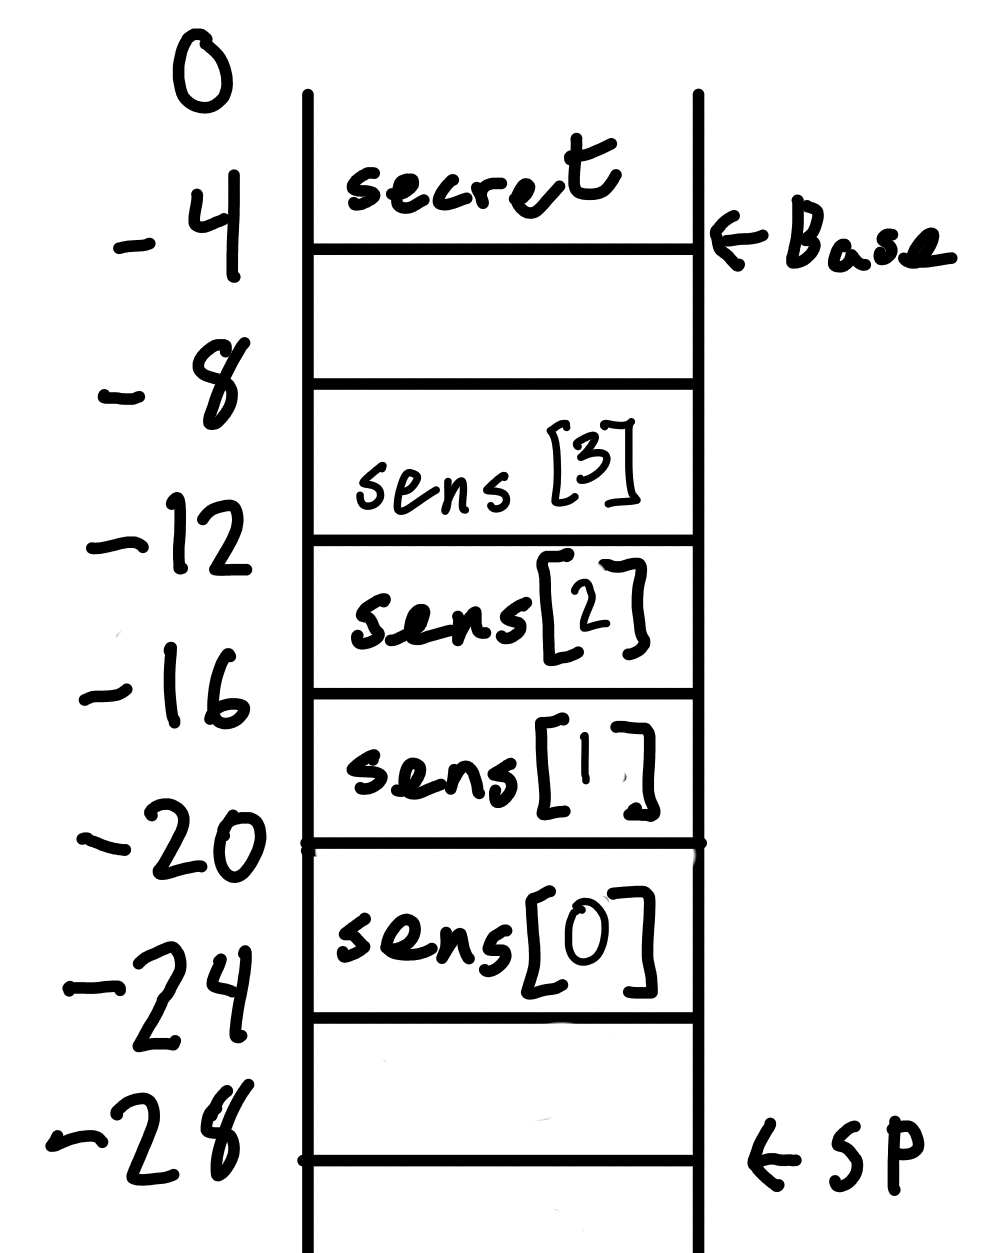
\includegraphics[width=\columnwidth]{stacklayout.png}
  \end{subfigure}

\caption{Example: Main}
\label{fig:main}
\end{figure}

Suppose that {\tt f} is not a (valid) C function at all, but an attacker seeking
to leak {\tt secret}! It might do so in a number of ways, shown as snippets of
assembly code in Figure \ref{fig:f}.
\apt{In (a,b), {\tt 12(sp)} maps to {\tt sensitive}, not {\tt secret} (I think!).
  It would be nice if (a) didn't have to push a frame (i.e. again by making publication
  just a global write) and if all the examples of {\tt f} were the same length, e.g.
  by adding {\tt nop}s.}

In Figure \ref{subfig:direct}, {\tt f} takes an offset from the stack
pointer, access {\tt secret}, and directly call {\tt publish} itself. But more
subtly, even if somehow prevented from outputting {\tt secret} directly, {\tt f}
instead return that value so that {\tt main} makes the call to {\tt publish},
as in Figure \ref{subfig:indirect}.

Beyond simply reading {\tt secret}, the attacker might overwrite {\tt sensitive}
with 42, guaranteeing that {\tt main} publishes its own secret unintentionally
(Figure \ref{subfig:integrity})!
Attacks of this kind do not violate {\tt main}'s confidentiality, but its
{\it integrity}.
And in Figure \ref{subfig:WBCF}, the attacker attempts to return to the
wrong instruction, thereby bypassing the check and publishing {\tt secret} regardless,
violating the program's {\it well-bracketed control flow} (WBCF.)

\begin{figure}
  \begin{subfigure}[b]{\columnwidth}
    \vspace{\abovedisplayskip}
    \begin{tabular}{r l | l}
      \labeledrow{100:}{addi sp,sp,-8}{\(\mathbf{alloc} ~ (-8,8)\)}
      \labeledrow{104:}{sd ra,0(sp)}{}
      \labeledrow{108:}{lw a0,12(sp)}{}
      \labeledrow{112:}{jal 200,ra}{\(\mathbf{call} ~ 200 ~ \{\mathtt{a0} ~ \emplist\}\)}
      \labeledrow{116:}{lw ra,0(sp)}{}
      \labeledrow{120:}{addi sp,sp,8}{\(\mathbf{dealloc} ~ (0,8)\)}
      \labeledrow{124:}{jalr ra}{\(\mathbf{return}\)}
    \end{tabular}
    \caption{Leaking {\tt secret} directly}
    \label{subfig:direct}
  \end{subfigure}  
  \begin{subfigure}[b]{\columnwidth}
    \vspace{\abovedisplayskip}
    \begin{tabular}{r l | l}
      \labeledrow{100:}{lw a0,12(sp)}{}
      \labeledrow{104:}{jalr ra}{\(\mathbf{return}\)}
    \end{tabular}
    \caption{Leaking {\tt secret} indirectly}
    \label{subfig:indirect}
  \end{subfigure}  
  \begin{subfigure}[b]{\columnwidth}
    \vspace{\abovedisplayskip}
    \begin{tabular}{r l | l}
      \labeledrow{100:}{li a5,42}{}
      \labeledrow{104:}{sw a5,4(sp)}{}
      \labeledrow{108:}{jalr ra}{\(\mathbf{return}\)}
    \end{tabular}
    \subcaption{Attacking {\tt sensitive}}
    \label{subfig:integrity}
  \end{subfigure}
  \begin{subfigure}[b]{\columnwidth}
    \vspace{\abovedisplayskip}
    \begin{tabular}{r l | l}
      \labeledrow{100:}{addi ra,ra,20}{}
      \labeledrow{104:}{jalr ra}{\(\mathbf{return}\)}
    \end{tabular}
    \subcaption{Attacking control flow}
    \label{subfig:WBCF}
  \end{subfigure}

  \caption{Assembly code for {\tt f} as an attacker}
  \label{fig:f}
\end{figure}

\apt{This para is a bit of an orphan.}
At the start of execution the program counter is 0 and the stack pointer -4 \apt{or is it 0?},
with the stack growing down. The functions {\tt f} and {\tt publish}
are at addresses 100 and 200, respectively.

\apt{Need a smoother transition here. Be explicit that we are now going to start considering the security
  state.}

Figure \ref{fig:exec1} shows how the program counter, stack pointer, and context
develop over several steps, with labels on the steps that allocate space and then make
a call. \(\xrightarrow{\overline{\psi}}\) transitions are written \(\downarrow \overline{\psi}\) in this diagram;
events are omitted.\apt{graphics on right of figure need to be keyed to corresponding steps.}

The first step  allocates words for {\tt secret}, {\tt sensitive}, and {\tt res}, as well
as two words for the return address. This will have the
effect of marking those bytes \(\object\), assuming they were previously
\(\unsealed\).

\begin{figure*}
  \begin{subfigure}[t]{.5\textwidth}
    \vskip 0pt
    \begin{tabular}{| l | l | l || l |}
      \hline
      Step & \(\PCname\) & \(\SP\) & \(\context\) \\
      \hline
      0 & 0 & 0 & \(V_0, \emplist\) \\
      \hline
      \multicolumn{4}{l}{\(\downarrow [\mathbf{alloc} ~ (-20,20)]\)} \\
      \hline
      1 & 4 & -20 & \(V_1 = V_0 \llbracket -20 \ldots -1, \mapsto \object \rrbracket\) \\
      \hline
      \multicolumn{4}{l}{\(\vdots\)} \\
      \hline
      4 & 16 & -20 & \(V_1, \emplist\) \\
      \hline
      \multicolumn{4}{l}{\(\downarrow [\mathbf{call} ~ 100 ~ \emplist ~ \emplist]\)} \\
      \hline
      5 & 100 & -20 & \(V_2 = V_1 [\mathtt{a0} \mapsto \unsealed],[(V_1, 20, -20)]\) \\
      \hline
      \multicolumn{4}{l}{\(\vdots\)} \\
      \hline
      \(n\) & ? & ? & \(V_2,[(V_1, 20, -20)]\) \\
      \hline
      \multicolumn{4}{l}{\(\downarrow [\mathbf{return}]\)} \\
      \hline
      \(n+1\) & 20 & -20 & \(V_1, \emplist\) \\
      \hline
    \end{tabular}
  \end{subfigure}
  \begin{subfigure}[t]{.4\textwidth}
    \vskip 0px
    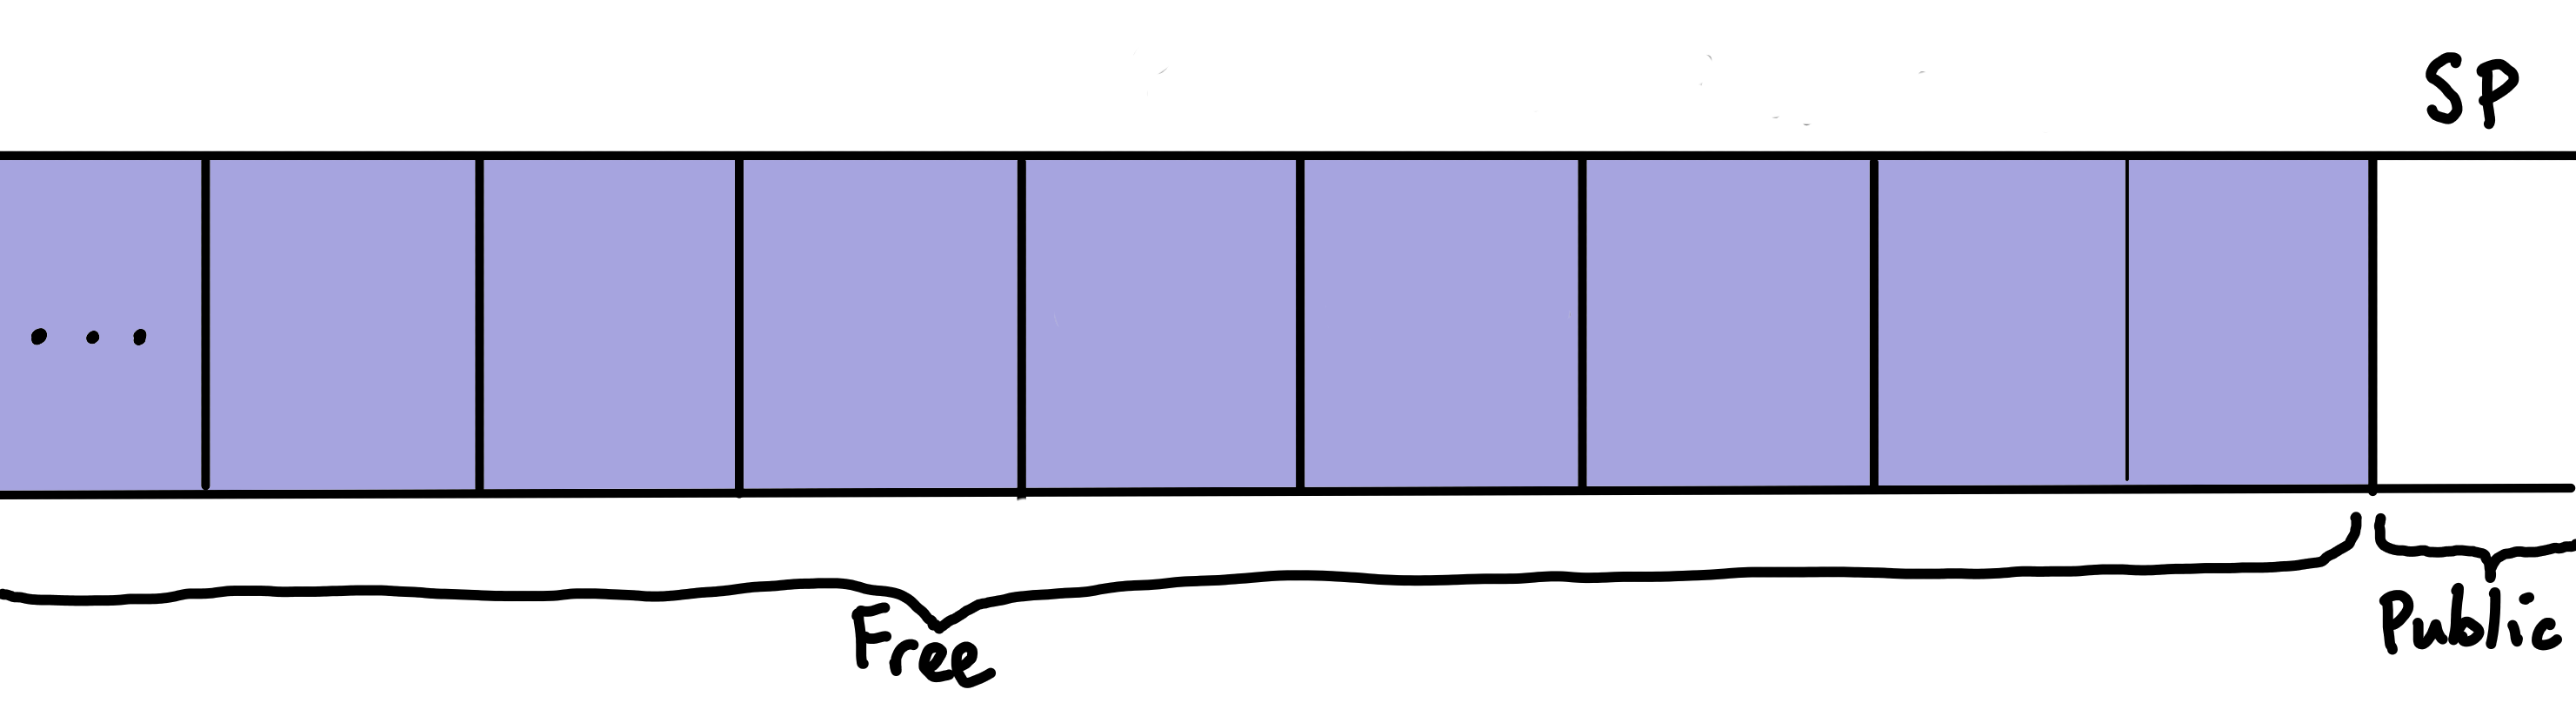
\includegraphics[width=\columnwidth]{stack1.png}
    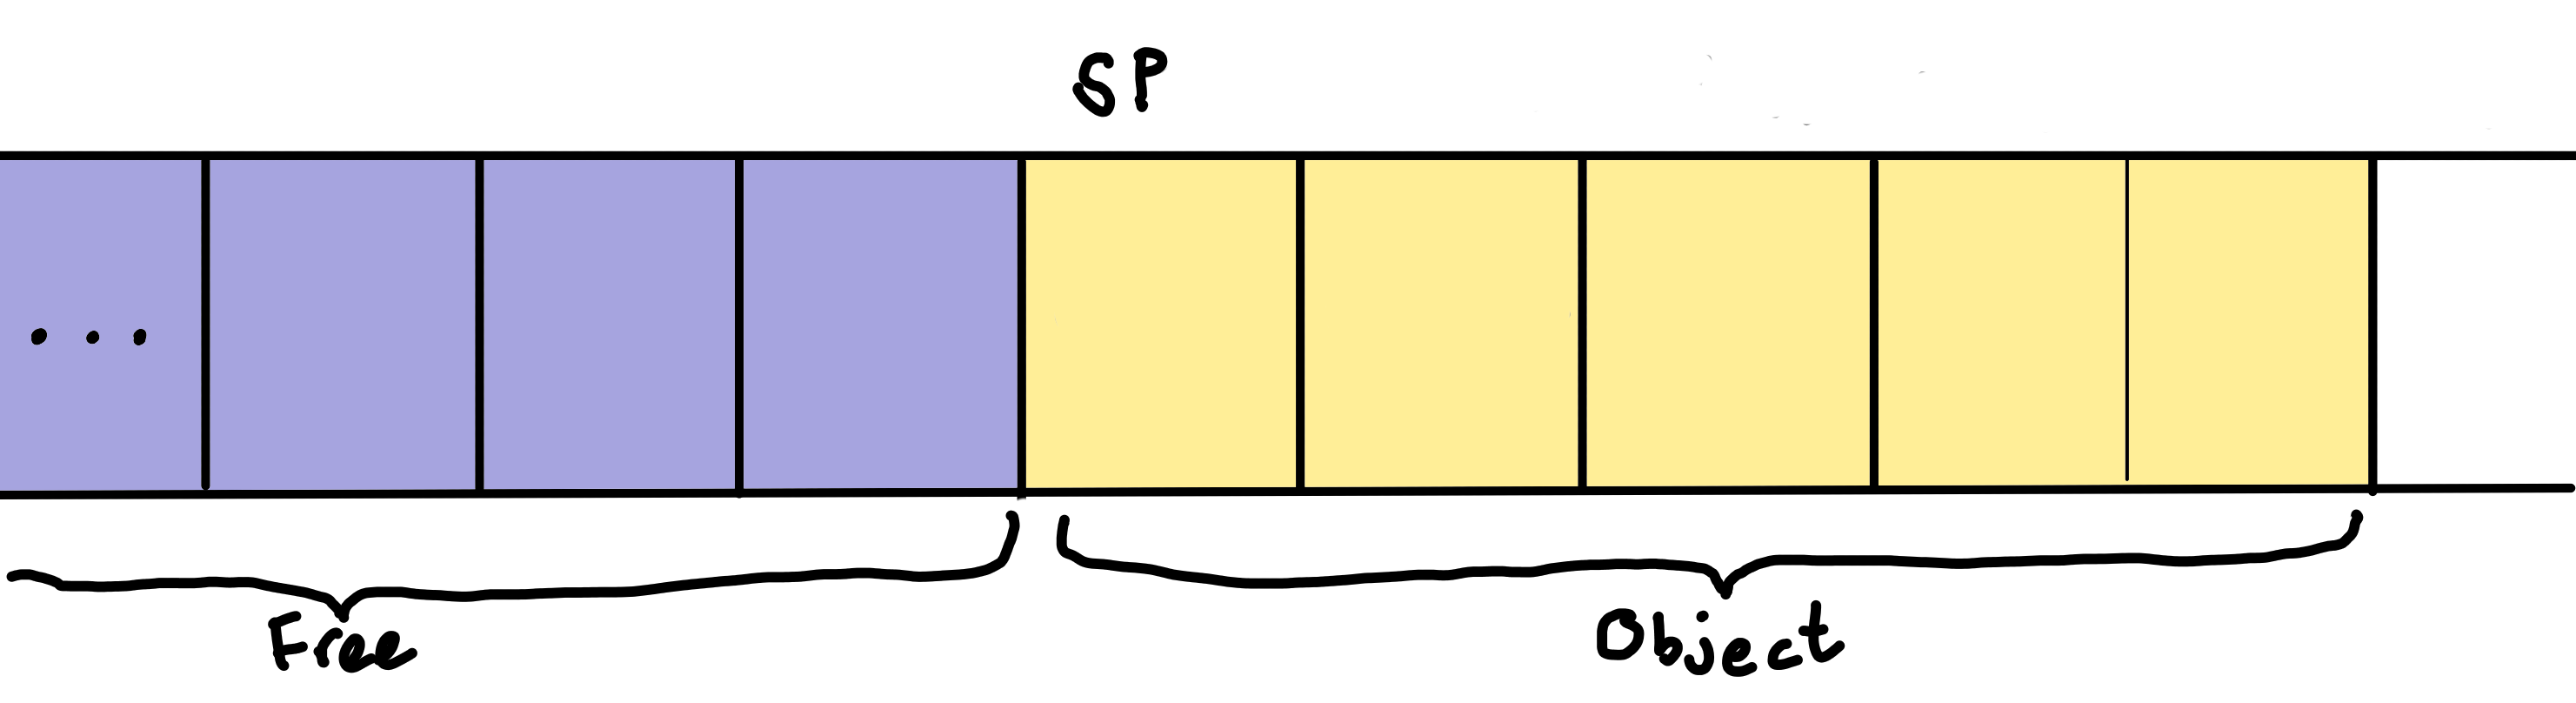
\includegraphics[width=\columnwidth]{stack2.png}
    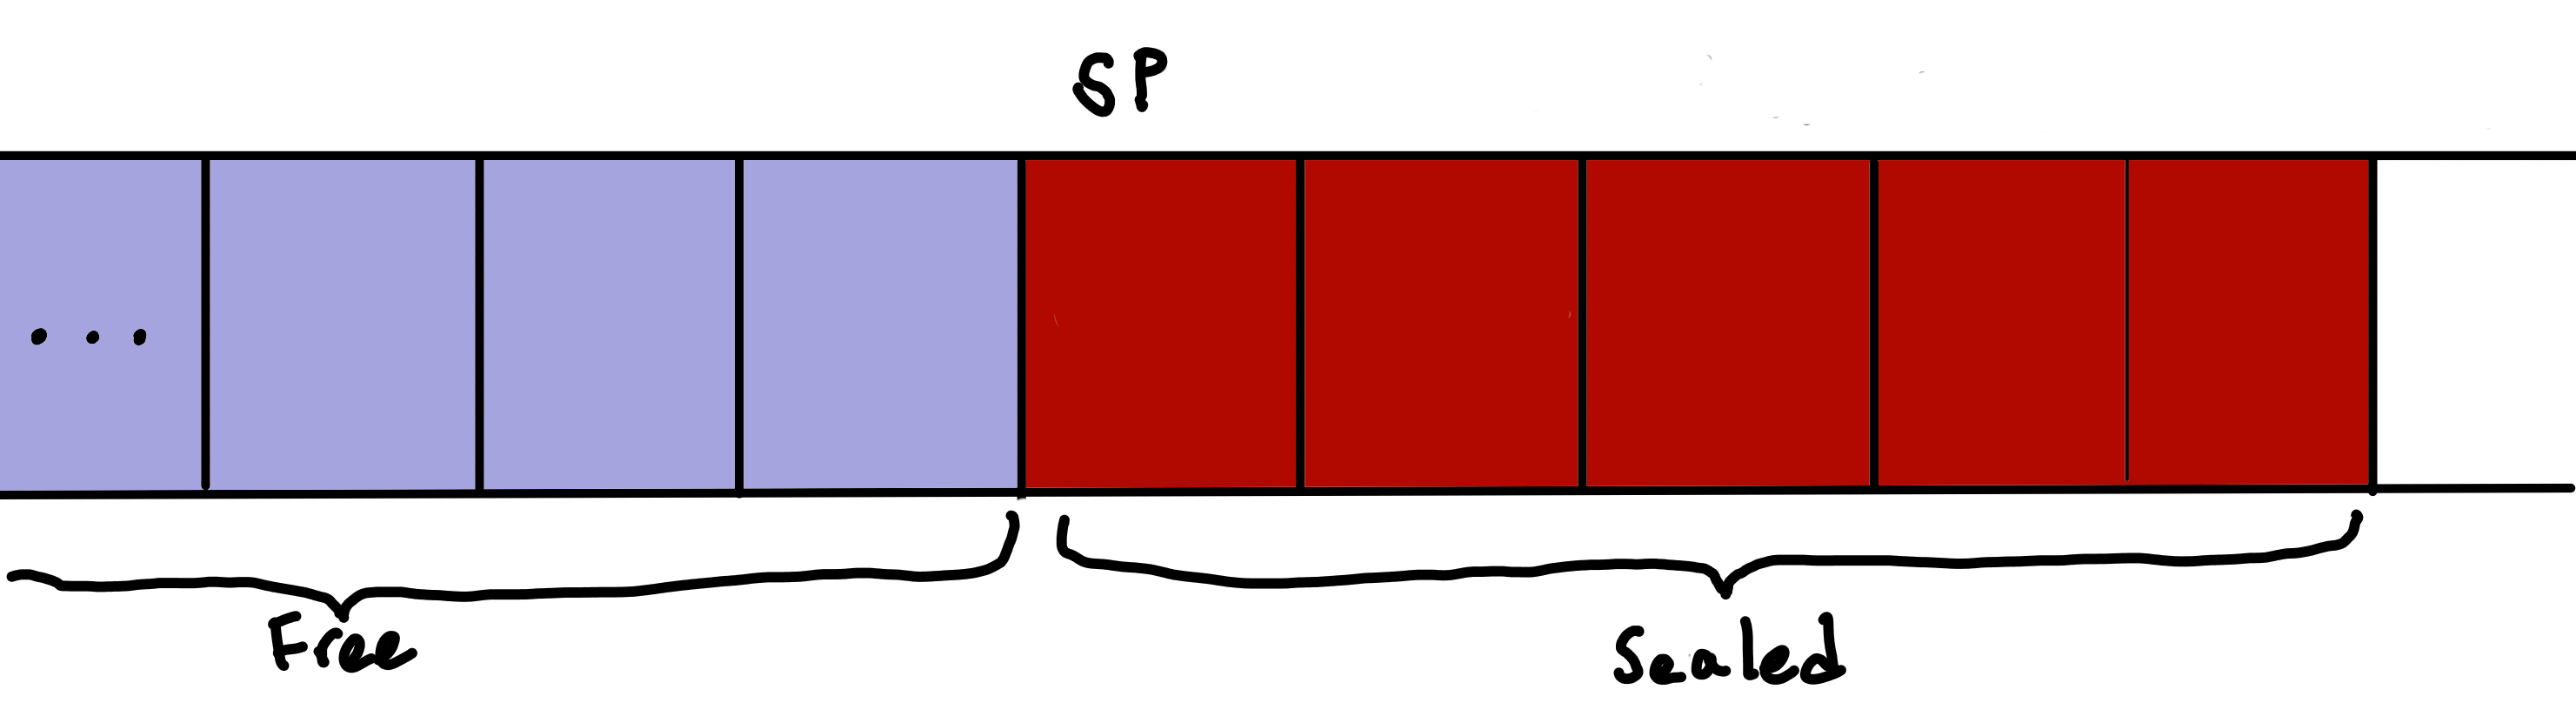
\includegraphics[width=\columnwidth]{stack3.png}
    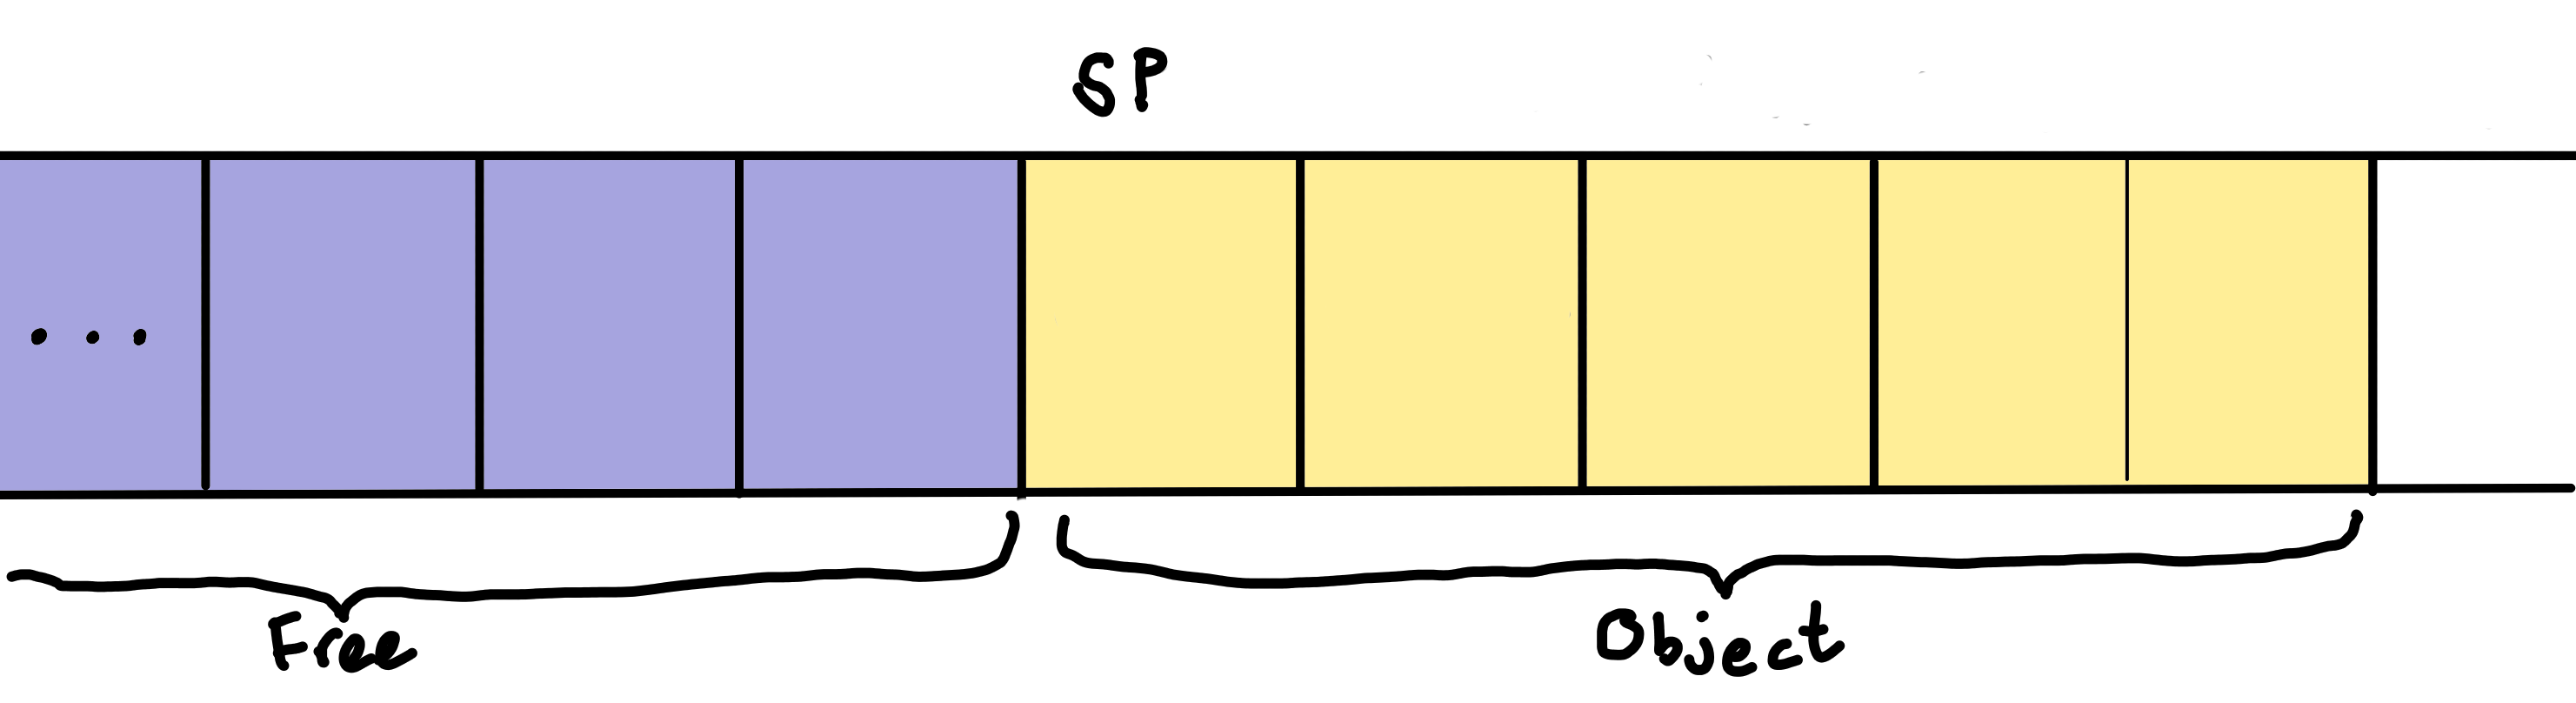
\includegraphics[width=\columnwidth]{stack4.png}
  \end{subfigure}

\caption{Execution through return from {\tt f}}
\label{fig:exec1}
\end{figure*}

On a call, the formerly active principal's record is pushed onto the inactive list.
Its return target is the return address of the call, 
and the stack pointer target is the stack pointer at the moment of call.
The callee's view is updated from the caller's such that all \(\object\) locations
become \(\sealed\). (In more complex settings, objects that are intentionally passed
to the callee will not get sealed, but for now we assume no sharing of memory between activations.)
For registers, \(\overline{\reg_{args}}\) tells us which registers are used as arguments,
in this case {\tt a0}. These are mapped to \(\public\), while any non-argument, caller-saved
registers are mapped to \(\unsealed\). All callee-save registers are always \(\sealed\) and
the program counter \(\public\), as they were initialized.

On step \(n\), {\tt f} returns, and we restore the topmost inactive principal,
{\tt main}'s principal. \apt{This $n$ is a bit mysterious. Again, if all the snippets
  were the same length, you could use a concrete number here.}
         
\apt{Need a bridging sentence here, along the lines of: ``Now we consider how to define desirable
  stack safety properties that rule out various kinds of bad behavior.''}

\paragraph*{Well-bracketed Control Flow}

But what if {\tt f} returns to an unexpected place (i.e. \(\PCname \neq 20\) or \(\SP \neq -24\))\apt{-20?},
as would be the case in attack (d)? Then it has violated the WBCF property.
This property can be phrased in terms of a single step: for every transition
labeled as a return, the program counter and stack pointer at the next state
match those recorded in the top pending activation. The table in Figure \ref{fig:exec1}
assumes that WBCF is followed.

\paragraph*{Stack Integrity}

Integrity is more complicated, and requires us to compare the state at the start of
the call to {\tt f} to that on return. Intuitively, the integrity of {\tt main}
is preserved if, when control returns to it, it can rely on any \(\sealed\) elements
to be identical to when it made the call.

In the case of the call from {\tt main} to {\tt f}, the \(\sealed\) elements are the
addresses -20 through -1 (allocated as private data) and callee-saved registers such as
the stack pointer and return address.
Note that the callee-saved registers may well have changed during the call---but if
so, the callee is obligated to restore them to their prior value.

One further caveat: it is possible that {\tt f} might overwrite {\tt main}'s data
in a way that is harmless---or that is rendered harmless by the enforcement mechanism!
\apt{This is still confusing, because the ``rendered harmless'' part applies just as much
  to the strict integrity we've been discussing up to now.}
This is the case in a lazy micro-policy\apt{presumes we've described these a bit in the introduction
  (which we should)}: the monitor permits the caller to write into the
callee's frame, but taints that write so that the callee cannot read it later without
triggering a failstop. In such a scenario we will consider a value {\it irrelevant}
if it could be replaced with any other value without changing the observable behavior
of the machine. More precisely, for a given state \(\mach\) and set of elements \(\components\),
we define a {\em \(\components\)-variant} state to be one agrees with \(\mach\) on every
element except those in \(\components\). The elements of \(\components\) are said to be
irrelevant in \(\mach\) if every variant state produces an equivalent trace
(see Section \ref{sec:events}.)

So, to define integrity, we need to know when a caller has been returned to;
this is the first state after the call in which the depth of the call stack
matches the state before the call. Integrity holds if, at that return state,
any element that is \(\sealed\) under the callee's view is either restored
to its original value or is irrelevant.

Returning to our example: at step 4, when {\tt main} makes its call to {\tt f},
the call stack in the context is empty. It makes its call, and at step 5, {\tt main}'s
frame, including {\tt secret} and {\tt sensitive}, is mapped to \(\sealed\) from the
perspective of {\tt f}. So, the next time the call stack is empty (implicitly, when
we have returned to {\tt main}), elements of that frame must either match their
values at step 4, or be irrelevant to future computation.\apt{picture?}

\paragraph*{Caller Confidentiality}

We treat confidentiality as a form of non-interference as well: the confidentiality of a caller
means that its callee's behavior is dependent only on publicly visible data,
not the caller's private state. \apt{Spell out the implications of this for initialization.}
As we saw in the examples, we must consider both the observable events
that the callee produces during the call and the changes that the callee makes to the state that might
affect the caller after the callee returns.

Consider the state \((\mach, (V_2,\sigma))\) at step 5. If we take a variant state over
the set of element(s) that are \(\sealed\) or \(\unsealed\) in \(V_2\),
{\it internal confidentiality} means
that, if we execute both states until they return, they will produce equivalent sequences
of events.

But, in Figure \ref{subfig:indirect}, we also saw an attacker that exfiltrated the secret
by reading it and then returning it, in a context where the caller would output the returned
value. In situations like this, we care about {\it return-time confidentiality}.
In that case, we would identify that in our original execution, {\tt a0} changed between
the call and return, being set to the value of {\tt secret}. But in a variant state,
{\tt secret} might have a different value, and so will {\tt a0} at the return.
This difference, found by comparing the initial and final states of both executions,
indicates that {\tt a0} is corrupted. Return-time confidentiality means that
an element that is corrupted in this way must be irrelevant.

Together, these definitions encompass the confidentiality of the caller from the callee.\apt{picture?}

\paragraph*{Callee Confidentiality}

Although we presented our initial example from the perspective of the caller, a callee
may also have data that must be kept secret from its caller. Consider a callee that makes
a privileged system call to obtain a secret key, and uses that key to perform a specific
task. An untrustworthy or erroneous caller might attempt to read the key out of the callee's
memory after return.

We model this as nearly dual to caller integrity: the callee's secrets are those
values that it has stored in \(\unsealed\) elements. So, callee confidentiality means that
at the state following the callee's return, any element that was \(\unsealed\) under the
callee's view either retains its original value or is irrelevant.

\paragraph*{The Hierarchy of Stack Safety}

The forms of stack safety described above are largely independent of one another, and
can potentially be enforced separately in various combinations. This is important, because
many existing enforcement mechanisms enforce only some of the stack safety
properties. Stricter enforcement may have greater performance impacts, leading to decisions
about trade-offs between different degrees of stack safety.

In principal, these properties can exist in any combination, but in practice we see examples
of certain combinations that form a hierarchy. Many enforcement techniques focus purely on
well-bracketed control flow. Stack canaries aim to prevent certain attacks on the return
address, and shadow stacks with protection (e.g. Return Address Defender \cite{Chiueh2001RAD})
to enforce it completely.

Others combine this protection with some degree of memory protection,
chiefly focusing on integrity. Skorstengaard et al. \cite{SkorstengaardSTK} characterize stack
safety as the combination of WBCF and {\it local state encapsulation} (LSE), and prove that their
capability-based enforcement satisfies both. LSE corresponds to integrity, plus some degree of
confidentiality.\apt{Be more explicit.}  They offer a fully abstract overlay semantics, which formalizes WBCF and LSE
together as a safe-by-construction abstract machine. That machine does not allow a callee to
read or write its caller's frame, but might allow it to read data that is left behind below
the caller's frame, which is weaker than our full caller confidentiality and rules out
callee confidentiality entirely. Georges et al. \cite{Georges22:TempsDesCerises} correct
both limitations.

\paragraph*{Moving Forward}

In the next section we will define traces and their (hyper-)properties.
Then in Section \ref{sec:facts} we will define a mechanism to make assertions
about what will happen on a future return, and Section \ref{sec:props} will use these
to give the formal definitions of integrity and confidentiality.

\section{Events and Traces}
\label{sec:events}

We abstract over the events that can be observed in the system, defining them
only as a set \(\OBSS\) that contains at least the element \(\tau\), the silent
event. Other events might represent certain function calls (i.e., system calls)
or writes to special addresses representing mmapped regions.
A {\em trace} is a nonempty, finite or infinite sequence
of events, ranged over by \(\obsT\).
We use ``\(\notfinished{}{}\)'' to represent ``cons'' for traces, reserving ``::''
for list-cons.

We write that execution from a state produces an observation trace
\(\mach,\context \hookrightarrow \obsT\) as follows, coinductively:

\judgmenttwo{\((\mach,\context) \stepstounder{} (\mach',\context',\obs)\)}
            {\((\mach',\context') \hookrightarrow \obsT\)}
            {\((\mach,\context) \hookrightarrow \notfinished{\obs}{\obsT}\)}

We define another relation that takes a trace until we have returned from the
active principal.
We write this \(d \downarrow (\mach,\context) \hookrightarrow \obsT\), where
\(d\) is the depth of the current call.

\judgment{\(|\sigma| < d\)}
         {\(d \downarrow (\mach,(V,\sigma)) \hookrightarrow \tau\)}

\judgmenttwobrlong{\((\mach,(V,\sigma)) \stepstounder{} (\mach',\context',\obs)\)}
                  {\(|\sigma| \geq d\)}
                  {\(d \downarrow (\mach',\context') \hookrightarrow \obsT\)}
                  {\(d \downarrow (\mach,(V,\sigma)) \hookrightarrow \notfinished{\obs}{\obsT}\)}

\paragraph*{Observational Similarity}

We say that two event traces $\obsT_1$ and $\obsT_2$ are {\em similar},
written \(\obsT_1 \eqsim \obsT_2\), if the sequence of non-silent events
is the same. That is, we compare up to deletion of \(\tau\) events.

\begin{minipage}{.4\columnwidth}
  \judgment{}{\(\obsT \eqsim \obsT\)}
\end{minipage}
\begin{minipage}{.4\columnwidth}
  \judgment{\(\obsT_1 \eqsim \obsT_2\)}
           {\(\notfinished{\obs}{\obsT_1} \eqsim \notfinished{\obs}{\obsT_2}\)}
\end{minipage}

\begin{minipage}{.4\columnwidth}
  \judgment{\(\obsT_1 \eqsim \obsT_2\)}
           {\(\notfinished{\tau}{\obsT_1} \eqsim \obsT_2\)}
\end{minipage}
\begin{minipage}{.4\columnwidth}
  \judgment{\(\obsT_1 \eqsim \obsT_2\)}
           {\(\obsT_1 \eqsim \notfinished{\tau}{\obsT_2}\)}
\end{minipage}

\paragraph*{Variants and Irrelevant Values}

Two states are variants with respect to a set of elements, \(\components\),
if they agree on the value of every element not in \(\components\). Our
notion of non-interference involves comparing the traces of such
\(\components\)-variants. We use this to define sets of irrelevant elements.

\definition Machine states \(\mach\) and \(\nach\) are {\em \(\components\)-variants},
written \(\mach \approx_\components \nach\), if, for
all \(\component \not \in \components\), \(\mach[\component] = \nach[\component]\).

\definition An element set \(\components\) in state \((\mach,\context)\) contains
irrelevant values, written \((\mach,\context) \parallel \components\), if for all
\(\nach\) such that \(\mach \approx_{\components} \nach\), if 
\((\mach,\context) \hookrightarrow \obsT\) and
\((\nach,\context) \hookrightarrow \obsT'\), then
\(\obsT \eqsim \obsT'\).

\section{Facts Abouts Calls and Returns}
\label{sec:facts}

Here we define some logical operations to reason about the behavior of the
system over time. These have a temporal-logic flavor, as they reflect
the expected behavior of the system in the future, after a possible return.

\paragraph*{On-return}

The intuition behind integrity (below) is that a caller may expect its
sealed data to be unchanged when control returns to it. In fact, the callee
may overwrite such data---when the data are found in callee-saved registers
this is perfectly legal---as long as it either restores it, or has some guarantee
that its changes will not impact the caller.

We start by defining a second-order logical operator
\(d \uparrow P\), pronounced ``\(P\) holds on return from depth \(d\),''
where \(P\) is a predicate on machine states. This is a coinductive relation
similar to ``weak until'' in temporal logic---it also holds if the program never
returns from depth \(d\).

\judgmenttwo[Returned]
            {\(|\sigma| < d\)}
            {\(P ~ (\mach,(V,\sigma))\)}
            {\((d \uparrow P) ~ (\mach, (V,\sigma))\)}

\judgmenttwobrlong[Step]
                  {\(|\sigma| \geq d\)}
                  {\((d \uparrow P) ~ (\mach', \context')\)}
                  {\((\mach, (V,\sigma)) \stepstounder{\overline{\psi}} (\mach', \context',\obs)\)}
                  {\((d \uparrow P) ~ (\mach, (V,\sigma))\)}

Similarly, for confidentiality, we will want to compare pairs of future states,
so we give a binary equivalent, \(d \Uparrow R\), where
\((\mach,\context) ~ (d \Uparrow R) ~ (\mach',\context')\) holds if \(R\) holds on the
first states that return from depth \(d\) after \((\mach,\context)\) and \((\mach',\context')\),
respectively. Once again, \(\Uparrow\) is coinductive.

\judgmenttwobrlong[Returned]
            {\(|\sigma_1| < d\)}
            {\(|\sigma_2| < d\)}
            {\((\mach_1,(V_1,\sigma_1)) ~ R ~ (\mach_2,(V_2,\sigma_2))\)}
            {\((\mach_1,(V_1,\sigma_1)) ~ (d \Uparrow R) ~ (\mach_2,(V_2,\sigma_2))\)}

\judgmenttwobrlong[Left]
              {\(|\sigma_1| \geq d\)}
              {\((\mach_1,(V_1,\sigma_1)) \stepstounder{\overline{\psi}} (\mach_1',\context_1',\obs)\)}
              {\((\mach_1',\context_1') ~ (d \Uparrow R) ~ (\mach_2,(V_2,\sigma_2))\)}
              {\((\mach_1,(V_1,\sigma_1)) ~ (d \Uparrow R) ~ (\mach_2,(V_2,\sigma_2))\)}

\judgmenttwobrlong[Right]
              {\(|\sigma_2| \geq d\)}
              {\((\mach_2,(V_2,\sigma_2)) \stepstounder{\overline{\psi}} (\mach_2',\context_2',\obs)\)}
              {\((\mach_1,(V_1,\sigma_1)) ~ (d \Uparrow R) ~ (\mach_2,\context_2')\)}
              {\((\mach_1,(V_1,\sigma_1)) ~ (d \Uparrow R) ~ (\mach_2,(V_2,\sigma_2))\)}

\section{Properties}
\label{sec:props}

We now finally have everything we need to formalize our definitions for stack safety.
Figure \ref{fig:oprules} gives the operation rules for all of the operations we've described
so far.

\begin{figure}

  \judgmentbr[Alloc]
             {\(b = \mach[\SP] + \mathit{off}\)}
             {\(V' = V \llbracket \addr \mapsto \sealed |
               b \leq a < b+\mathit{sz} \land V ~ \addr = \unsealed \rrbracket\)}
             {\(Op ~ \mach ~ (\mathbf{alloc} ~ \mathit{off, sz}) ~ (V,\sigma) = (V',\sigma)\)}

  \judgmentbr[Call]
             {\(\psi = \mathbf{call} ~ \addr_{target} ~ \overline{\reg_{args}} ~ \overline{sa}\)}
             {\(V' = V \llbracket \reg \mapsto \unsealed | \reg \in \mathit{CLR} \rrbracket
               \llbracket \reg \mapsto \public | \reg \in \overline{\reg_{args}} \rrbracket\)}
             {\(Op ~ \mach ~ \psi ~ (V,\sigma) =
               (V',(V, \mach[\PCname]+4, \mach[\SP])::\sigma)\)}

  \judgment[Ret]
           {\(\sigma = (V,\addr_{ret},\addr_{sp})::\sigma'\)}
           {\(Op ~ \mach ~ \mathbf{return} ~ (\_, \sigma) = (V, \sigma)\)}
           
%\judgment[RetDef]
%         {\(\chi = \mathbf{return}\)}
%         {\(Cop ~ \chi ~ (V, \emplist) ~ \mach \triangleq
%           (V, \emplist)\)}

  \caption{Core operation rules for the simple system}
  \label{fig:oprules}
\end{figure}

\subsection{Well-bracketed Control Flow}

\definition A system enjoys {\it well-bracketed control flow} if 
\((\mach,(\_,(\_,\addr_{ret},\addr_{sp})) \stepstounder{\mathbf{return}} (\mach',\context,\obs)\)
implies \(\mach'[\PCname] = \addr_{ret}\) and \(\mach'[\SP] = \addr_{sp}\).

\vspace{\abovedisplayskip}

\apt{These explanations that relate the definitions back to the example snippets are
  great. They would be even better if you can find a way to put them in Section II,
  based on (less formal) definitions of the terms introduced here.}
  
Consider again the attack in Figure \ref{subfig:WBCF}: the attacker adds
20 to the return address and then returns, thus bypassing the check and publishing
{\tt secret}. During the call step, we record in the context that the return to the
caller should have the program counter at the next instruction (address 20) and the
stack pointer restored to address -20. When the return occurs, we see that in the
state following it, the program counter is 40---a violation of WBCF.

To demonstrate why WBCF also cares about the stack pointer, consider an attack which
returns with the stack pointer at -12 instead of -20. Now, compare the layout of the stack relative
to the stack pointer as it should be (top) to the one that results by increasing the
stack pointer before return (bottom):

\begin{tabular}{| l | l | l | l | l | l | l |}
  \multicolumn{3}{r}{\(\SP \downarrow\)} \\
  \hline
  & & res & sens & secr & ra & ra \\
  \hline
  \hline
  res & sens & secr & ra & ra & & \\
  \hline
\end{tabular}

\apt{I think it might be clearer just to have one row with the two different SP pointers
  (the proper one and the bad one) marked.}

\vspace{\abovedisplayskip}

In this scenario, when attempting to read {\tt sensitive}, {\tt main} will
read part of the return address, and then it will attempt to publish
{\tt res}, but instead will publish {\tt secret}!

There is an alternative foramlization of well-bracketed control flow using \(\uparrow\).

\definition For a machine state \(\mach\), let
\(ret ~ (\mach,\context) = \{\mach' \mid \mach'[\SP] = \mach[\SP] \land \mach'[\PCname] = \mach[\PCname]\}\).
\apt{Note: you'll get better spacing by using $\mid$ rather than $|$ in set comprehensions.}
A system enjoys  well-bracketed control flow if
\((\mach,\context) \stepstounder{\overline{\psi}} (\mach',(V,\sigma),\obs)\) where 
\(\mathbf{call} ~ \addr ~ \overline{\reg} ~ \overline{sa} \in \psi\) or
\(\mathbf{tailcall} ~ \addr ~ \overline{\reg} ~ \overline{sa} \in \psi\)
implies \(|\sigma| \uparrow ret(\mach')\).

\vspace{\abovedisplayskip}

\apt{Sudden appearance of $\mathbf{tailcall}$??}
Once again we can think about our example attack. When the call occurs,
we define a predicate \(ret ~ (\mach,\context)\) on states that holds when the program counter
and stack pointer have the appropriate values. Then we use apply the \(\uparrow\)
operator to this predicate with the depth of the call stack {\it after the call} and
the machine state {\it before the call}.

After the call, the size of the call stack, \(|\sigma|\), is one greater than it was before the call,
and if the callee makes further calls, it will continue to be incremented.
Similarly, each return will decrement it, until it is finally lower than in the
initial state. This is the return that matches the original call, and so
the resulting state is when we require \(ret(\mach)\) to hold.

\subsection{Integrity}

\definition Let \(\Delta(\mach,\mach')\) be the set of elements \(\component\)
such that \(\mach[\component] \not = \mach'[\component]\).

\definition Let \((\mach,\context)\) be a combined state with
\(\context = (V,\sigma)\), and
\(\components = \{\component \mid V ~ \component = \sealed\}\).
Let \(P ~ (\mach',\context')\) be a predicate that holds on a state
\(\Delta(\mach,\mach')\) is irrelevant in \((\mach', \context')\).\apt{Something is broken here!}
Then \(\mach\) enjoys {\it return-time integrity} if \(|\sigma| \uparrow P\) holds
on \((\mach,\context)\).

\definition A system enjoys {\it stack integrity} if, for all reachable states
\((\mach,\context)\) such that
\((\mach,\context) \stepstounder{\overline{\psi}} (\mach',\context',\obs)\) with
\(\mathbf{call} ~ \addr ~ \overline{\reg} ~ \overline{sa} \in \psi\) or
\(\mathbf{tailcall} ~ \addr ~ \overline{\reg} ~ \overline{sa} \in \psi\),
\((\mach',\context')\) enjoys return-time integrity.

\vspace{\abovedisplayskip}

The example in Figure \ref{subfig:integrity} modifies the value of {\tt sensitive},
which is \(\sealed\). At the call, we define the predicate \(P\), which holds on states
where any \(\sealed\) elements that changed since the call are all irrelevant.
As {\tt sensitive} is such an element (conveniently, the only one), the property
has not yet been violated at the returned state \((\mach,\context)\). To determine whether this
attack has violated stack integrity, we must consider an arbitrary variant state
\(\nach = \mach[\addr_{\mathtt{sensitive}} \mapsto \word]\) for some \(\word\).
The property is violated if the traces of \((\mach,\context)\) and \((\nach,\context)\)
differ.

In our case, {\tt publish} produces an observation, and if \(\word \not = 42\),
that observation in the trace from \((\nach,\context)\) will be {\tt res}, which is 0.
On the other hand, \((\mach,\context)\) will produce an event from {\tt secret},
which may differ. So, integrity is indeed violated.

\subsection{Caller Confidentiality}

\definition The {\em corrupted set} \(\bar{\Diamond}(\mach,\mach',\nach,\nach')\)
of four states treats \(\mach\) and \(\nach\) as the initial states and
\(\mach'\) and \(\nach'\) as their corresponding final states, and is the
set of elements that were corrupted between them. That is, the set of all elements
\(\component \in \Delta(\mach,\mach') \cup \Delta(\nach,\nach')\) such that
\(\mach'[\component] \not = \nach'[\component]\). ]\apt{Define first, explain after.}

\definition Let \((\mach,\context)\) be a state with \(\context = (V,\sigma)\), and
\(\components = \{\component \mid V ~ \component \in \{\sealed, \unsealed\}\}\).
Then \((\mach,\context)\) enjoys {\it internal confidentiality} with respect to \apt{??}
if, for any \(\nach\) that is a \(\components\)-variant of \(\mach\), we can take
\(|\sigma| \uparrow (\mach,\context) \hookrightarrow \obsT\) and
\(|\sigma| \uparrow (\nach,\context) \hookrightarrow \obsT'\) and have that
\(\obsT \simeq \obsT'\).

\definition Let \((\mach,\context)\) be a state with \(\context = (V,\sigma)\),
and \(\components = \{\component \mid V ~ \component \in \{\sealed, \unsealed\}\}\).
Let \(\nach\) be a \(\components\)-variant of \(\mach\).
Let \(R\) be a relation such that \((\mach_1,\context_1) ~ R ~ (\mach_2,\context_2)\)
if \(\bar{\Diamond}(\mach,\mach_1,\nach,\mach_2)\) is irrelevant in \((\mach_1,\context_1)\).
Then \((\mach,\context)\) enjoys {\it return-time confidentiality}
if, for any such \(\nach\), \((\mach,\context) ~ (|\sigma| \Uparrow R) ~ (\nach,\context)\).

\definition A system enjoys {\it caller confidentiality} if, for all reachable states
\((\mach,\context)\) such that
\((\mach,\context) \stepstounder{\overline{\psi}} (\mach',\context',\obs)\)
with \(\mathbf{call} ~ \addr ~ \overline{\reg} ~ \overline{sa} \in \psi\) or
\(\mathbf{tailcall} ~ \addr ~ \overline{\reg} \in \psi\),
\((\mach',\context')\) enjoys both internal and return-time confidentiality.

\vspace{\abovedisplayskip}

Confidentiality is more complicated. We begin with a state immediately following
a call. Let that be \((\mach,\context)\). We suppose an arbitrary variant state,
\((\nach,\context)\), which may vary any element that is \(\sealed\) or \(\unsealed\).
That is, any element that is not used legitimately to pass arguments. Caller confidentiality
therefore can be thought of as the callee's insensitivity to parts of its initial states
that are not part of the caller-callee interface.

In the example in Figure \ref{subfig:direct}, this variation will quickly result
in differing events, as {\tt publish} is called with arguments that may have different
values. This is clearly a violation of confidentiality, in the form of internal
confidentiality.

When the variants return, however, the situation becomes more complicated.
Consider Figure \ref{subfig:indirect}. The value of {\tt secret} is been extracted
and placed in {\tt a0}, the return value register. Suppose that we have \(\mach\)
and \(\nach\) as above, and they step, respectively, to \(\mach'\) and \(\nach'\),
which each follow a return. We must identify which elements of the state
contain leaked confidential data.

An element contains confidential data, according to the definition of non-interference, 
if it differs between the states. But some of those data belong to the original
elements which are accessible to the caller and may now influence future execution
legitimately. We are looking specifically for those elements that have {\it changed}
from call to return, and that vary between the variants. As with integrity, we then
must determine whether those leaks actually translate into events. If the set of
such elements is not irrelevant, confidentiality is violated.

\subsection{Callee Confidentiality}

\definition Let \((\mach,\context)\) be a state with \(\context = (V,\sigma)\), and
\(\components = \{\component \mid V ~ \component = \unsealed\}\).
Let \(P\) be a predicate that holds on a state \((\mach',\context')\) if
\(\mach' ~ \parallel ~ \Delta(\mach,\mach') \cap \components\).
Then \(\mach\) enjoys {\it post-return confidentiality} if \(|\sigma| \downarrow P\) holds.

\definition A system enjoys {\it callee confidentiality} if, for all reachable states
\((\mach,\context)\) such that \((\mach,\context) \stepstounder{\overline{\psi}} (\mach',\context',\obs)\)
with \(\mathbf{call} ~ \addr ~ \overline{\reg} ~ \overline{sa} \in \psi\) or
\(\mathbf{tailcall} ~ \addr ~ \overline{\reg} ~ \overline{sa} \in \psi\),
\((\mach',\context')\) enjoys post-return confidentiality
with respect to \(\context\).

\section{Shared Memory}

%We can extend our basic machine to support public memory allocations that can
%be accessed by anyone until they are deallocated on their owner's return,
%using the \(\mathbf{alloc\_pub}\) operation. This behaves identically to
%\(\mathbf{alloc\_priv}\) except that it marks the locations \(\public\).
%For example, consider the following code:

%{\tt
%  void g() \{

%  ~ ~ int x[3];

%  ~ ~ int y;

%  ~ ~ h(\&x);
    
%  \}
%}

%Here we have allocated several arrays and variables; {\tt y}
%will behave as normal with \(\mathit{alloc\_priv}\), but {\tt x} has its
%address taken and passed to another function. That function might do anything at
%all to {\tt x}, and we have to decide whether it can be said to violate stack
%safety. A reasonable default is to assume that any address-taken local should be
%public, while {\tt y} is still private.

%In the likely event that the space for the return address, {\tt x}, and {\tt y}
%are all allocated in a single step, that step needs multiple labels to capture
%that they are not all private. Its label would instead be:
%\[\begin{split}
%& \psi = [\mathbf{alloc\_priv} ~ (20,4); \\
%  & \mathbf{alloc\_pub} ~ (16,12) ; \mathbf{alloc\_priv} ~ (4,4)]
%\end{split}\]

%Allocating public objects affects the call stack very similarly to private ones,
%but instead of treating them as \(\sealed\) they become \(\public\). This makes these
%regions of memory able to transmit information between caller and callee without
%violating the stack safety properties. Note that there is no way to seal a location
%once it has become \(\public\); only when {\tt g} returns will the memory allocated
%to {\tt x} be available for private use.

%\judgmentbr{\(b = \mach[\SP] - \mathit{off}\)}
%           {\(V' = V \llbracket \addr \mapsto \public |
%             b \leq a < b+\mathit{sz} \land V ~ \addr = \unsealed \rrbracket\)}
%           {\(Pop ~ (\mathbf{alloc\_pub} ~ \mathit{off, sz}) ~ (V,\sigma) ~ \mach \triangleq
%             (V',\sigma)\)}

\subsection{Stack Arguments}

So far, we have not dealt with arguments spilled onto the stack, variadic arguments,
or arguments that are passed by reference without their addresses being taken
explicitly (i.e., structs and arrays passed directly.) Consider the simplest case,
where a function has more than 8 arguments and therefore must (in RISC-V) spill one
to the stack.

{\tt
  void main() \{

  ~ f(1,2,3,4,5,6,7,8,9);

  ~ g(42);
  
  \}
}

\vspace{\abovedisplayskip}

\begin{tabular}{r l | l}
  \labeledrow{0:}{addi sp,sp,-12}{\(\mathbf{alloc} ~ (-12,12)\)}
  \labeledrow{4:}{sd ra,4(sp)}{}
  \labeledrow{8:}{li a5,9}{}
  \labeledrow{12:}{sd a5,0(sp)}{}
  \labeledrow{16:}{li a7,8}{}
  \dots \\
  \labeledrow{48:}{jal 100,ra}{\(\mathbf{call} ~ \{\mathtt{a0-a7}\} ~ \{(\SP,0,4)\}\)}
  \labeledrow{52:}{li a0,42}{}
  \labeledrow{56:}{jal 200,ra}{\(\mathbf{call} ~ \{\mathtt{a0}\} ~ \emplist\)}
  \dots \\
\end{tabular}

Under a typical calling convention, the callee expects the ninth argument to
be passed to it at bottom of the caller's frame, so the caller allocates extra
space for it. Then the call to {\tt f} identifies that we expect a range of four
bytes from the stack pointer to be passed as an object instead of sealed.

So we must refine our call operation to make use of the information that we have about
which memory contain arguments, \(\overline{sa}\). \(\overline{sa}\) is a set of
triples of a register, an offset from the value of that register, and a size.
We first define the helpful set \(\mathit{passed} ~ \overline{sa} ~ \mach\),
then extend the call operation to keep all objects in \(\mathit{passed}\) marked
as \(\object\) and seal everything else.
%
\[\mathit{passed} ~ \overline{sa} ~ \mach \triangleq
\bigcup_{(\reg,b,o) \in \overline{sa}} \{\mach[\reg]+i | b \leq i < b+o\}\]
%
\judgmentbrbr[]
             {\(\psi = \mathbf{call} ~ \addr_{target} ~ \overline{\reg_{args}} ~ \overline{sa}\)}
             {\(V' = V \llbracket \reg \mapsto \unsealed | \reg \in \mathit{CLR} \rrbracket
               \llbracket \reg \mapsto \public | \reg \in \overline{\reg_{args}} \rrbracket\)}
             {\(V'' = V'\llbracket \addr \mapsto \sealed | V' ~ \addr = \object \land \addr \not \in (\mathit{passed} ~ \overline{sa} ~ \mach) \rrbracket\)}
             {\(Op ~ \mach ~ \psi ~ (V,\sigma) =
               (V',(V, \mach[\PCname]+4, \mach[\SP])::\sigma)\)}

The remaining definitions are unchanged. Now a stack-spilled argument can be allocated
and remain accessible in the callee, while its memory is sealed for calls that do not
use that memory as an argument.

This same structure works for pass-by-reference arguments: we know from the type of
the called function which register it expects to hold the address of a given object,
and the size of that object. In this case the offset will always be 0.

When the callee in such a scenario makes a call of its own, the objects passed to it
will in turn be sealed---unless it passes them on, which can happen with pass-by-reference
arguments!

\subsection{Provenance, Capabilities, and Protecting Objects}

What if we want to express a finer-grained notion of safety, in which
such objects are protected unless the function that owns them intentionally
passes a pointer to them?

In order to express such a property, we need our machine to carry some notion
of {\it pointer provenance}---a distinction between a pointer that is intended to
point to a given object, and non-pointer integers as well as pointers to other objects.
Then \(\mathit{passed}\) should recursively identify all objects that
are reachable transitively from valid pointers in registers and accessible memory;
these keep their \(\object\) status, while those that are not reachable become \(\sealed\).
         
\bibliographystyle{IEEEtran}
\bibliography{bcp.bib,local.bib}

\end{document}
